\documentclass[UTF8, 11pt, a4paper]{ctexart}
\usepackage{tikz}
\usetikzlibrary{math} % tikzmath
\begin{document}

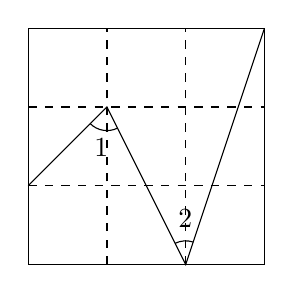
\begin{tikzpicture}
\draw (0,0)--(3,0)--(3,3)--(0,3)--cycle;
\draw[dashed](1,0)--(1,3) (2,0)--(2,3) (0,1)--(3,1) (0,2)--(3,2);
\draw (0,1)--(1,2) --(2,0)--(3,3);

\coordinate (P12) at (1, 2);
\tikzmath{
    \r = 0.3;
    \start = 180 + atan(1);
    \endd = 360 - atan(2);
    \shift{x} = \r * cos(\start);
    \shift{y} = \r * sin(\start);
}
\coordinate (start_1) at ([shift={(\shift{x}, \shift{y})}] P12);
\draw (start_1) arc (\start:\endd:\r);

\coordinate (P20) at (2, 0);
\tikzmath{
    \r = 0.3;
    \start = atan(3);
    \endd = 180 - atan(2);
    \shift{x} = \r * cos(\start);
    \shift{y} = \r * sin(\start);
}
\coordinate (start_2) at ([shift={(\shift{x}, \shift{y})}] P20);
\draw (start_2) arc (\start:\endd:\r);

\node at ([shift={(0.14,-0.3)}] start_1) {1};
\node at ([shift={(-0.1,0.3)}] start_2) {2};

\end{tikzpicture}

\end{document}